\documentclass{article}

\usepackage{algorithmic}
\usepackage{basiccolors}
\usepackage{amsmath}
\usepackage{amssymb}
\usepackage{graphicx}
\usepackage{theorem}

\newcommand{\myA}{{\cal A}}
\newcommand{\myS}{{\cal S}}
\newcommand{\myR}{{\mathbf R}}
\newcommand{\Dmat}[4]{D_{#1 #2 #3 #4}}
\newcommand{\Mmat}[4]{M_{#1 #2 #3 #4}}
\newcommand{\IAmat}[4]{I^\textrm{A}_{#1 #2 #3 #4}}
\newcommand{\IBmat}[4]{I^\textrm{B}_{#1 #2 #3 #4}}

%% matrices for the formulation with quadratic instead on n^4-tables
%% use as follows:
%% \DTmat{a}{b}
%% \MTmat{a}{b}{i}{k}
%% \IATmat{a}{b}{i}
%% \IBTmat{a}{b}{k}

\newcommand{\DTmat}[2]{D(#1,#2)}  
\newcommand{\MTmat}[4]{M^{{#1}^l {#2}^l}(#3,#4)}
\newcommand{\IATmat}[3]{I^{{#1}^l {#2}}_\textrm{A}(#3)}
\newcommand{\IBTmat}[3]{I^{{#1} {#2}^l}_\textrm{B}(#3)}


\newcommand{\pInLoop}[3]{p_{#1}^\textrm{loop}(#2|#3)}
\newcommand{\pInLoopA}[2]{\pInLoop{A}{#1}{#2}}
\newcommand{\pInLoopB}[2]{\pInLoop{B}{#1}{#2}}

\newcommand{\PsiA}[1]{\Psi^\textrm{A}_{#1}}
\newcommand{\PsiB}[1]{\Psi^\textrm{B}_{#1}}


\newcommand{\thetaOne}{\theta_1}
\newcommand{\thetaTwo}{\theta_2}

\newtheorem{theorem}{Theorem}[section]
\newtheorem{lemma}[theorem]{Lemma}
\newtheorem{proposition}[theorem]{Proposition}
\newtheorem{corollary}[theorem]{Corollary}

\newenvironment{proof}[1][Proof]{\begin{trivlist}
\item[\hskip \labelsep {\bfseries #1}]}{\end{trivlist}}
\newenvironment{definition}[1][Definition]{\begin{trivlist}
\item[\hskip \labelsep {\bfseries #1}]}{\end{trivlist}}
\newenvironment{example}[1][Example]{\begin{trivlist}
\item[\hskip \labelsep {\bfseries #1}]}{\end{trivlist}}
\newenvironment{remark}[1][Remark]{\begin{trivlist}
\item[\hskip \labelsep {\bfseries #1}]}{\end{trivlist}}

\newcommand{\qed}{\nobreak \ifvmode \relax \else
      \ifdim\lastskip<1.5em \hskip-\lastskip
      \hskip1.5em plus0em minus0.5em \fi \nobreak
      \vrule height0.75em width0.5em depth0.25em\fi}


\title{LocARNA Next Generation}

\begin{document}

\maketitle

We describe a new variant of Sankoff's simultaneous folding and
alignment algorithm that promises higher accurcy compared to existing
fast Sankoff-like algorithms and supports the known heuristic
accellerations as well as significant novel structural
sparsification. For sequences of length $n$, the final algorithm runs
in $O(n^2)$ compared to $O(n^6)$ of the original Sankoff algorithm.

Like PMcomp we simplify the algorithm by using a base-pair based
energy model, where base pair weights are derived from McCaskill base
pair probabilities. However, instead of scoring only the energy of the
consensus structure, we predict one structure for each sequence and
score its energy. Like in Sankoff the predicted structures and the
alignment are required to be compatible and the total score is the sum
of the single energies and a sequence alignment score.
  
This simplified variant of the algorithm is much closer to the
original formulation than PMcomp and promises to predict structures
more accurately. In the same way as PMcomp, it significantly reduces
the computational cost of the Sankoff-algorithm and is amenable to the
same optimizations as introduced by LocARNA.

Furthermore, we present a novel structural sparsification strategy
that in combination with the known sparsification by base pair
probability (as used by LocARNA, FoldalignM, RAF, Lara) reduces the
time complexity to $O(n^2)$. The idea of this strategy is to compute,
for each base pair $(i,j)$ and position $k$, the conditional
probability that $k$ is member of the loop $(i,j)$. Then, the DP
algorithm is limited to consider only 'probable' bases.

\subsection*{Related Work}

\Red{\bf Remarks about RAF:} RAF combines structural sparsity from
single sequences dot-plots with alignment sparsity from sequence
alignment. We should be able to implement the latter sparsification
quite easily in LocARNA/LocARNAng.  (In the LocARNA code, there is a
currently unused class for computing sequence alignment edge
probabilities already.) The sequence alignment sparsity works
orthogonal to our new structural sparsification idea.

RAF furthermore composes its score from features based on these
probabilities (i.e. base pair and alignment edge probs, unpaired and
unaligned probabilities). In RAF, the weights of these features are
automatically learned (max-margin model). This seems to cause the much
improved accuracy of RAF over LocARNA. It would be interesting to use
learning and/or the new scoring idea in LocARNA and the new LocARNA
derivative.

\section{Methods}

\subsection{Preliminaries}

Consider two sequences $A$ and $B$ with associated base pair
probability matrices $P^A$ and $P^B$, respectively. 

A sequence alignment $\myA$ consists of a set of (mis)matches written
as pairs $(i,k)$, where $i$ is a position in $A$, and $k$ a position
in $B$.

The \emph{extended consensus secondary structure} (ecss) \Red{(term?
  alignment of structures???)} $\myS$ for an alignment $\myA$ consists
of a set of tuples $(ij;kl)$, $(ij,-)$, and $(-,kl)$, where $(i,j)$ is
a base pair on sequence $A$ and $(k,l)$ is a base pair on sequence
$B$, \Red{missing: $(ij,-)$ implies (by def of consensus structure)
  that $(i,j)$ is an inner base pair of a 2-loop (or on the top-level
  and unbranched, 'pseudo-base pair match'), $(-,kl)$ implies ...,
  Note: there is a common super-tree of the two (implied) single
  structures. }

A consensus structure $\myS$ is compatible with the alignment $\myA$
iff
\begin{enumerate}
\item for all $(ij;kl)\in\myS$: $(i,k)\in\myA$ and $(j,l)\in\myA$
\item \Red{``for each (ij,-), the base pair i,j and the loop of which
    i,j is inner base pair is deleted in $\myA$''.}
\end{enumerate}

Furthermore, $\myA_s$ is the set of alignment edges in $\myA$ that are
not structurally matched, i.e. 
\begin{displaymath}
  \myA_s = \{ (i,k)\in\myA \mid \nexists (ij;kl)\in\myS \text{ and }
  \nexists (ji;lk)\in\myS
  \}.
\end{displaymath}

The score of $(\myA,\myS)$ is given by
\begin{equation}
  \label{eq:simscore}
  \sum_{(ij;kl)\in\myS} (\PsiA{ij}+\PsiB{kl})
  + \sum_{(ij;-)\in\myS} \PsiA{ij}
  + \sum_{(-;kl)\in\myS} \PsiB{kl}
  + \sum_{(i,k)\in\myA_s} \sigma(A_i,B_k) 
  - N_{\textrm{gap}}\gamma,
\end{equation}
where $\PsiA{ij}$ and $\PsiB{kl}$ are base pair scores (see below),
$\sigma:\{A,C,G,U\}^2\to\myR$ is the similarity score for
(mis)matches, $\gamma$ is the gap score parameter and
$N_{\textrm{gap}}$ is the number of insertions and deletions in the
alignment $\myA$.  \Red{MM: Why do we have no alignment score for the
  matched edges? Maybe better $\sum_{(i,k)\in\myA} \sigma(A_i,B_k)$
  than $\sum_{(i,k)\in\myA_s} \sigma(A_i,B_k)$? This would only require
  to modify the last recursion case of $M_{ijkl}$ to incorporate
  (mis)matching costs.}

\subsection{Basic Algorithm}
We define four matrices
\begin{itemize}
\item $\Dmat{i}{j}{k}{l}$ := best score of an subalignment/ecss pairs of $A$ and $B$
  in ranges ${i..j}$ and ${k..l}$
\item $\Mmat{i}{j}{k}{l}$ := best score of an subalignment/ecss pairs
  of $A$ and $B$ in ranges ${i..j}$ and ${k..l}$, where all outermost
  base pairs in the ecss are matched
\item $\IAmat{i}{j}{k}{l}$ := best score of an subalignment/ecss pairs
  of $A$ and $B$ in ranges ${i..j}$ and ${k..l}$, where the ecss
  contains (i'j';-) as outermost xxx and every position in $A$ within
  $i+1..i'$ and $j'..j-1$ is aligned to a gap. (\Red{we need to define
    outermost for ecss such that (i'j') is outermost in implied
    structure of A and there is no (k'l') that 'encloses' (i'j') via
    the alignment. For such purpose, define the eccs forrest. Then,
    (i'j',-) has to be the single root of the ecss forrest. Note that
    due to definition of alignment/ecss compatibility (i'j',-) in ecss
    implies that all bases of the corresponding loop (where $(i',j')$
    is interior base pair) are deleted.}
\item $\IBmat{i}{j}{k}{l}$ := \Red{``symmetric''}.
\end{itemize}

\begin{align}
  \Dmat{i}{j}{k}{l} &= \max
  \begin{cases}
    \Mmat{i}{j}{k}{l}\\
    \IAmat{i}{j}{k}{l}\\
    \IBmat{i}{j}{k}{l}
  \end{cases}\\
  %
  \Mmat{i}{j}{k}{l} &= \max
  \begin{cases}
    \Mmat{i}{j-1}{k}{l-1} + \sigma(j,l)\\
    \Mmat{i}{j-1}{k}{l} + \gamma\\
    \Mmat{i}{j}{k}{l-1} + \gamma\\
    \max_{pq} \Mmat{i}{p-1}{k}{q-1} + \Dmat{p+1}{j-1}{q+1}{l-1} + \PsiA{pj} + \PsiB{ql}
  \end{cases}\\
  %
  \IAmat{i}{j}{k}{l} &= \max
  \begin{cases}
    \IAmat{i}{j-1}{k}{l} + \gamma\\
    \max_p (p-i+2)\gamma + \Dmat{p+1}{j-1}{k}{l} +  \PsiA{pj}
  \end{cases}\\
  %
  \IBmat{i}{j}{k}{l} &= \max
  \begin{cases}
    \IBmat{i}{j}{k}{l-1} + \gamma\\
    \max_q (q-k+2)\gamma + \Dmat{i}{j}{q+1}{l-1} +  \PsiB{ql}   
  \end{cases}
\end{align}

\Red{Note in recursion of $\IAmat{i}{j}{k}{l}$, $(p-i+2)\gamma$ could
  be equivalently replaced by $\IAmat{i}{p-1}{j}{j}$.}

\Red{
Remarks:
\begin{itemize}
\item
  Once can use structural sparsity as in LocARNA by considering only ``significant'' base pairs,
  which reduces time complexity from $O(n^6)$ to $O(n^4)$.
\item Note that all recursion cases recure to entries with the same
  left ends $i,k$ or entries $\Dmat{i}{j}{k}{l}$ that are enclosed by
  ``significant'' base pairs $(i+1,j-1)$ and $(k+1,l-1)$ respectively.
  Therefore, one can furthermore limit space requirements to $O(n^2)$
  as in LocARNA.
\item Furthermore for all matrices, it is sufficient to compute only
  entries $ijkl$, where significant base pairs $(i',j')$ and $(k',l')$
  exist in respective $P^A$ and $P^B$, such that $i'=i-1$, $k'=k-1$,
  $j<j'$, and $l<l'$.
\item Affine gap cost and strucural locality should be possible (TODO!).
\end{itemize}
}
\subsection{Basic Algorithm 2D detailed}
This is a formulation of the algorithm in terms of 2D matrices which
is equivalent to the previous one but much closer to the actual
implementation. It is also more detailed, giving the base cases, the
domains of the matrices, as well as visualizations of the recursion.

We define the following matrices:
\begin{itemize}
\item $\DTmat{a}{b}$ := best score of an subalignment/ecss pairs of $A$ and $B$
  in ranges ${i..j}$ and ${k..l}$
\item $\MTmat{a}{b}{i}{k}$ := best score of an subalignment/ecss pairs
  of $A$ and $B$ in ranges ${a^l+1..i}$ and ${b^l+1..k}$, where all outermost
  base pairs in the ecss are matched
\item $\IATmat{a}{b}{i}$ := best score of an subalignment/ecss pairs
  of $A$ and $B$ in ranges ${a^l+1..i}$ and ${b^l+1..b^r-1}$, where
  the ecss of this part contains some (i'j';-) with $a^l<i'<j'<a^r$ as
  outermost xxx and every position in $A$ within $a^l+1..i'$ and $j'..i-1$ is
  aligned to a gap. (\Red{we need to define outermost for ecss such
    that (i'j') is outermost in implied structure of A and there is no
    (k'l') that 'encloses' (i'j') via the alignment. For such purpose,
    define the eccs forrest. Then, (i'j',-) has to be the single root
    of the ecss forrest. Note that due to definition of alignment/ecss
    compatibility (i'j',-) in ecss implies that all bases of the
    corresponding loop (where $(i',j')$ is interior base pair) are
    deleted.}
\item $\IBTmat{a}{b}{k}$ := \Red{``symmetric''}.
\end{itemize}
\paragraph{base cases}
\begin{align}
  &\MTmat{a}{b}{a^l}{b^l}=0\\
  &\MTmat{a}{b}{i}{b^l}=(i-a^l)\gamma \text{ for all }i\in \{a^l+1,\dots,a^r-1\}\\
  &\MTmat{a}{b}{a^l}{k}=(k-b^l)\gamma \text{ for all }k\in \{b^l+1,\dots,b^r-1\}\\
  &\IATmat{a}{b}{a^l}=\IBTmat{a}{b}{b^l}=-\infty
\end{align}
\paragraph{recursion}
we compute values for all $a\in P^A$, $b\in P^B$, $i$, $k$
with $a^l<i<a^r$, $b^l<j<b^r$ as follows
\begin{align}
  \DTmat{a}{b} &= \max
  \begin{cases}
    \MTmat{a}{b}{a^r-1}{b^r-1}\\
    \IATmat{a}{b}{a^r-1}\\
    \IBTmat{a}{b}{b^r-1}
  \end{cases}\label{recursionD}\\
  %
  \MTmat{a}{b}{i}{k} &= \max
  \begin{cases}
    \MTmat{a}{b}{i-1}{k-1} + \sigma(i,k)\\
    \MTmat{a}{b}{i}{k-1} + \gamma\\
    \MTmat{a}{b}{i-1}{k} + \gamma\\
    \max_{\substack{a'\in P^A,b'\in P^B\\\text{s.t. } a'^r=i, b'^r=k}}\limits \MTmat{a}{b}{a'^l-1}{b'^l-1} + \DTmat{a'}{b'} + \tau(a',b')
  \end{cases}\label{recursionM}\\
  %
  \IATmat{a}{b}{i} &= \max
  \begin{cases}
    \IATmat{a}{b}{i-1} + \gamma\\
    \max_{a'\in P^A\text{ s.t.} a'^r=i}\limits (a'^l-a^l+1)\gamma + \DTmat{a'}{b} +  \PsiA{a'}
  \end{cases}\label{recursionIA}\\
  %
  \IBTmat{a}{b}{k} &= \max
  \begin{cases}
    \IBTmat{a}{b}{k-1} + \gamma\\
    \max_{b'\in P^B\text{ s.t.} b'^r=k}\limits (b'^l-b^l+1)\gamma +
    \DTmat{a}{b'} + \PsiA{b'}
  \end{cases}\label{recursionIB}
\end{align}
The recursions are visualized in Fig~\ref{}.
\begin{figure}
  \centering
  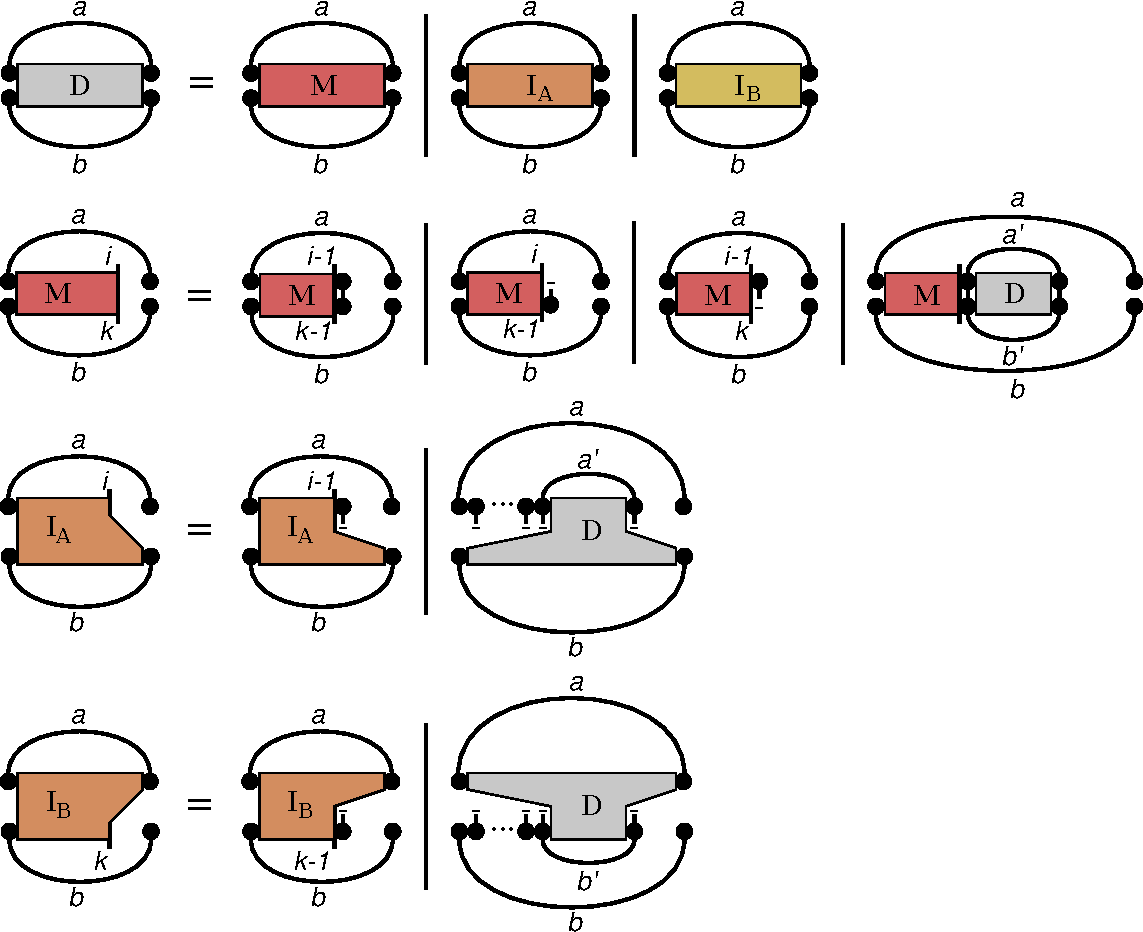
\includegraphics[width=\linewidth]{Figs/recursion}
  \caption{Visualization of the recursions
    \ref{recursionD}, \ref{recursionM},
    \ref{recursionIA}, and \ref{recursionIB}.}
  \label{fig:maximally_extended}
\end{figure}

\paragraph{evaluation order}
The following pseudocode shows in what order the tables can be
computed such that at any point in time only $O(n^2)$ space is
required.
\begin{algorithmic}
\FORALL {$x$ from $|A|$ to $1$ s.t. $\exists a\in P^A $ with $ a^l=x$}
  \FORALL {$y$ from $|B|$ to $1$ s.t. $\exists b\in P^B $ with $ b^l=y$}
    \STATE compute entire matrix $M^{xy}$
    \FORALL {$a\in P^A$ with $a^l=x$}
      \STATE compute entire matrix $I_A^{xb}$
    \ENDFOR
    \FORALL {$b\in P^B$ with $b^l=y$}
      \STATE compute entire matrix $I_B^{ay}$
    \ENDFOR
    \FORALL {$a\in P^A$, $b\in P^B$ with $a^l=x$,$b^l=y$ }
      \STATE compute $\DTmat{a}{b}$
    \ENDFOR
    \STATE free memory of matrices $M^{xy}$ and all $I_A^{xb}$,$I_B^{ay}$
  \ENDFOR
\ENDFOR
\end{algorithmic}

\subsection{Novel structural sparsification}

We consider a probability $\pInLoop{X}{k}{(i,j)} := \Pr[\text{$k$ in
  loop closed by $(i,j)$ in structure of $X$} \mid \text{$(i,j)$ base
  pair of $X$}]$ ($X\in\{A,B\}$).  See Exparna-P draft. Note:
immediately enclosed unpaired bases and right ends of inner bases are
'in loop' (that is the same definition that we need for
ExpARNA-P. Right ends are included to handle adjacent loops in
multi-loops correctly.).

For all matrices, we compute entries $ijkl$ if and only if there are
base pairs $(i',j')$ and $(k',l')$ in respective $P^A$ and $P^B$ such
that the following sparsity considitions are satisfied.
\begin{align}
  & i'=i-1, k'=k-1, j<j',\text{ and }l<l', and \label{eq:startpoints}\\
  & P^A(i',j')\geq \thetaOne\text{ and }P^B(k',l')\geq \thetaOne  \label{eq:theta-one} \\
  & \pInLoopA{j}{(i',j')} \geq \thetaTwo\text{ and  }\pInLoopB{l}{(k',l')} \geq \thetaTwo\label{eq:theta-two}.
\end{align}
The first two restrictions were already introduced before in LocARNA, whereas
the third one is new. 

\subsection{Complexity}

Recall: As argued before, there are at most $1/\thetaOne$ base pairs
$P^A(i,j)\geq \thetaOne$ for a fixed i. Therefore, there are only
$O(n)$ many base pairs $(i',j')$ satisfying condition~$(\ref{eq:theta-one})$.

\begin{proposition}
  \label{prop:sparsity}
  For a fixed $j$, there are only $O(1)$ base pairs $(i',j')$, such
  that all three sparsity conditions are satisfied.
\end{proposition}

\begin{proof}
  The probability $p(j,i',j'):=\Pr[\text{$j$ in loop closed by
    $(i',j')$ in structure of $A$}]$ is the joint probability
  $\Pr[\text{$(i',j')$ base pair of $A$ and $j$ in loop closed by
    $(i',j')$}]$. Therefore,
  $p(j,i',j')=P^A(i',j')\pInLoopA{j}{(i',j')} \geq
  \thetaOne\thetaTwo$.  For a fixed $j$, the events being in different
  loops are disjoint. Therefore $\sum_{(i',j')} p(j,i',j') \leq
  1$. Thus, there are at most $\frac{1}{\thetaOne\thetaTwo} \in O(1)$
  base pairs $(i',j')$ such that the conditions are satisfied.
\end{proof}

\begin{theorem}
  There are only $O(n^2)$ matrix entries that satisfy the sparsity conditions. 
\end{theorem}

\begin{proof}
  Let the sparsity conditions
  (\ref{eq:startpoints},\ref{eq:theta-one},\ref{eq:theta-two}) hold
  for $i$,$j$,$k$,$l$,$i'$,$j'$,$k'$, and $l'$.  Due to
  proposition~\ref{prop:sparsity} and $i=i'+1$, there are $O(n)$ many
  combinations $i',i,j$. Analogously there are $O(n)$ combinations
  $k',k,l$ and therefore $O(n^2)$ combinations $i',k',i,j,k,l$ satisfying
  the conditions.
\end{proof}

\begin{corollary}
  The time and space complexity of the sparsified algorithm is $O(n^2)$.
\end{corollary}

Recall that (as in LocARNA) each entry is computed in constant time
due to Condition $(\ref{eq:theta-one})$.

\Red{
Remarks:
\begin{itemize}
\item Previous approaches can not use this kind of sparsification,
  since they don't keep track of the enclosing base pair in the single
  structures but only enclosing base pairs of the consensus structure.
  This implies that in a state of the algorithm, we can't know the
  current loop of the single structure and therefore cannot filter
  based on the correct probability $\pInLoop{X}{k}{(i,j)}$.
\end{itemize}
}

\end{document}
